% =====================================================================
% Plantilla de respuestas · Tarea Computacional · IMT2220 (2026-2)
% =====================================================================
% Cómo usarla:
%   1. Completen el número de grupo y los integrantes (más abajo).
%   2. Reemplacen cada \pendiente por su desarrollo y su respuesta.
%   3. Las figuras que guarden desde sus notebooks van en la carpeta figuras/.
%   4. Compilen con pdfLaTeX (en Overleaf es el compilador por defecto) o con LuaLaTeX.
%
% En Overleaf: New Project > Upload Project y suban el .zip con esta carpeta.
% Pueden borrar estos comentarios y las cajas de "Indicaciones" cuando terminen.
\documentclass{article}
\usepackage{plantilla}
\graphicspath{{figuras/}}
\settitulo{Tarea Computacional}

% ---------------------------------------------------------------------
% Datos del grupo
% ---------------------------------------------------------------------
\newcommand\grupo{N}   % <-- número del grupo
\integrantes{%
  Nombre Apellido 1 \\
  Nombre Apellido 2 \\
  Nombre Apellido 3}

% Marca para lo que falta por completar (búsquenla con Ctrl+F antes de entregar)
\newcommand\pendiente{{\color{gris90}\itshape [Escriban aquí su desarrollo y su respuesta.]}}

\begin{document}

\portada[Grupo \grupo]

% =====================================================================
\seccionsinnumero{Indicaciones para usar esta plantilla}
% =====================================================================

\begin{nota}[Indicaciones]
  Esta plantilla es recomendada para resolver la tarea (aunque pueden utilizar cualquier otro formato mientras cumplan con lo solicitado). 
  Pueden reemplazar cada \pendiente{} por su desarrollo.
  Al final de este archivo hay ejemplos de cómo escribir ecuaciones, incluir figuras y tablas. Borren esa página antes de entregar.
\end{nota}

Algunas recomendaciones
\begin{itemize}
  \item \textbf{Desarrollo.} Justifiquen cada paso: no basta con el resultado. Cuando usen un resultado de clases, menciónenlo.
  \item \textbf{Resultados numéricos.} Reporten los valores que se piden (normas, residuos, $J(\theta)$, etc.) con 3 o 4 cifras significativas e indiquen de qué celda del notebook salen. (Esto no es estrictamente necesario, pero sí recomendado.)
  \item \textbf{Figuras.} Guárdenlas desde el notebook con \code{plt.savefig("figuras/nombre.png", dpi=200, bbox\_inches="tight")}, súbanlas a la carpeta \code{figuras/} (para que puedan añadirlas aquí) y comenten lo que se ve en ellas.
\end{itemize}
\despueslista

% =====================================================================
\problema{Reconstrucción de una imagen}
% =====================================================================

\seccion{(a) Mínimos cuadrados}

\begin{enumerate}[label=\roman*., widest=iii]
  \item \textbf{Gradiente y matriz Hessiana de $J_0$.}

  \pendiente

  \item \textbf{$H_{J_0}$ es semidefinida positiva y todo punto crítico es un mínimo global.}

  \pendiente

  \item \textbf{Unicidad o infinitos minimizadores.}

  \pendiente
\end{enumerate}
\despueslista

\seccion{(b) Reconstrucción}

\begin{enumerate}[label=\roman*., widest=ii]
  \item \textbf{Implementación.} Reporten $\norm{x_0}_2$, $\max_i \abs{x_{0,i}}$ y $\norm{Ax_0 - b}_2$, muestren lado a lado $b$ y $x_0$, y respondan las preguntas.

  \pendiente

  \item \textbf{Explicación.}

  \pendiente
\end{enumerate}
\despueslista

\seccion{(c) Regularización de Tikhonov}

\begin{enumerate}[label=\roman*., widest=iv]
  \item \textbf{Gradiente, Hessiana y único minimizador global.}

  \pendiente

  \item \textbf{Descomposición de $\ip{x_\lambda}{v_i}$ y cota del aporte del ruido.}

  \pendiente

  \item \textbf{Interpretación.}

  \pendiente

  \item \textbf{Implementación.} Completen la tabla y comparen las reconstrucciones.

  \begin{table}[H]
    \centering
    \begin{tabular}{>{\filatabla}l c c}
      \toprule[0.8bp]
                           & $\norm{x}_2$ & $\norm{Ax - b}_2$ \\
      \midrule[0.4bp]
      $x_0$                &              &                   \\
      $\lambda = 10^{-3.5}$ &             &                   \\
      $\lambda = 10^{-2.5}$ &             &                   \\
      $\lambda = 1$        &              &                   \\
      \bottomrule[0.8bp]
    \end{tabular}
    \caption{Norma y residuo de cada reconstrucción.}
    \label{tab:ridge}
  \end{table}

  \pendiente
\end{enumerate}
\despueslista

\seccion{(d) Píxeles dañados}

\begin{enumerate}[label=\roman*., widest=iii]
  \item \textbf{$\tilde{\eta} = \eta + (\tilde{b} - b)$ e interpretación de sus sumandos.}

  \pendiente

  \item \textbf{$\norm{\tilde{b} - b}_2$ y comparación de $\norm{\tilde{\eta}}_2$ con $\delta$.}

  \pendiente

  \item \textbf{¿Por qué fracasa la reconstrucción? ¿Bastaría con aumentar $\lambda$?}

  \pendiente
\end{enumerate}
\despueslista

\seccion{(Bonus) Mínimos cuadrados ponderados}

\pendiente

% =====================================================================
\problema{Red neuronal con dos capas ocultas}
% =====================================================================

\seccion{(a) Derivada de la sigmoide}

\pendiente

\seccion{(b) Función de pérdida y su gradiente}

\pendiente

\seccion{(c) Implementación y verificación del gradiente}

Reporten $\theta_0$, $J(\theta_0)$ y el error máximo $E$.

\begin{table}[H]
  \centering
  \begin{tabular}{>{\filatabla}c r r r}
    \toprule[0.8bp]
    Parámetro & Fórmula de (b) & $D_j$ & Diferencia \\
    \midrule[0.4bp]
    $a_1$ & & & \\
    $b_1$ & & & \\
    $a_2$ & & & \\
    $b_2$ & & & \\
    $v$   & & & \\
    $c$   & & & \\
    \bottomrule[0.8bp]
  \end{tabular}
  \caption{Gradiente en $\theta_0$: fórmulas de (b) y diferencias centradas.}
  \label{tab:gradiente}
\end{table}

\pendiente

\seccion{(d) Descenso del gradiente}

\pendiente

\seccion{(e) Parámetros encontrados}

\pendiente

\seccion{(f) Sensibilidad del entrenamiento}

\begin{enumerate}[label=\roman*., widest=ii]
  \item \textbf{Tamaño del paso.}

  \pendiente

  \item \textbf{Distintas inicializaciones.}

  \pendiente
\end{enumerate}
\despueslista

\seccion{(g) Datos de otra función}

\begin{enumerate}[label=\roman*., widest=ii]
  \item \textbf{Entrenamiento.}

  \pendiente

  \item \textbf{Monotonía, cotas y por qué la red no puede aproximar $\tilde{f}$.}

  \pendiente
\end{enumerate}

% =====================================================================
\clearpage\markright{}
\seccionsinnumero{Ejemplos de uso (borren esta sección antes de entregar)}
% =====================================================================

\seccion{Ecuaciones}

Una ecuación destacada se escribe entre \code{\textbackslash[} y \code{\textbackslash]}:
\[ \nabla J_0(x) = 2A^T(Ax - b). \]
Para varias líneas alineadas, usen \code{align*}:
\begin{align*}
  J_\lambda(x) &= \norm{Ax - b}_2^2 + \lambda \norm{x}_2^2 \\
               &= x^T (A^T A + \lambda I) x - 2 (A^T b)^T x + b^T b.
\end{align*}
La plantilla define \code{\textbackslash norm\{x\}}, \code{\textbackslash abs\{x\}}, \code{\textbackslash ip\{u\}\{v\}} (producto interno $\ip{u}{v}$), \code{\textbackslash R} ($\R$) y \code{\textbackslash diag}.

\seccion{Figuras}

Guarden la figura desde el notebook en la carpeta \code{figuras/} e inclúyanla así:
\begin{figure}[H]
  \centering
  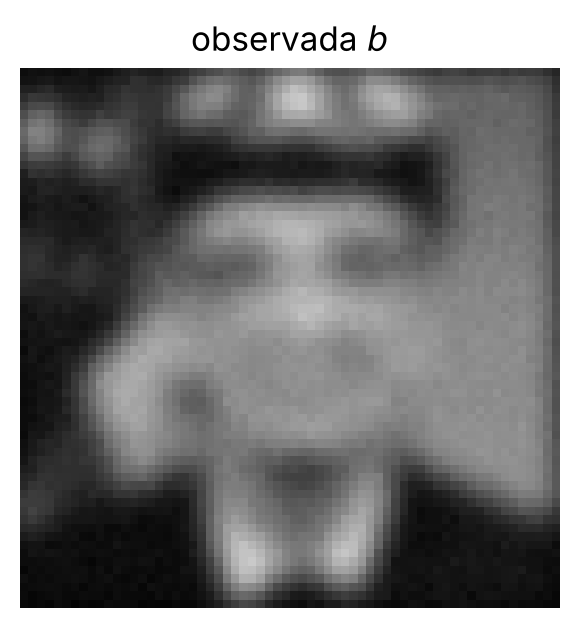
\includegraphics[width=6cm]{ejemplo_b.png}
  \caption{Imagen observada $b$ (ejemplo con los datos de la pauta).}
  \label{fig:ejemplo}
\end{figure}
Para referirse a ella, escriban \code{Figura\textasciitilde\textbackslash ref\{fig:ejemplo\}}: Figura~\ref{fig:ejemplo}.

\seccion{Cajas de comentarios}

\begin{nota}[Observación]
  Si quieren destacar un comentario, usen el entorno \code{nota}.
\end{nota}

\end{document}
